\section{Qualitative Analysis - Quasi-Free Scattering $^{12}$C(p,2p)$^{11}$B}
Until the S444 experiment in 2020 CALIFA consisted out of a prototype frame filled with up to 64 CsI(Tl) crystals. The geometric coverage was therefore poor. For the S444 experiment CALIFA got its final frame and was fully filled in the forward barrel and 35\%filled in the iPhos region, CEPA was not installed yet. With these improvements it was possible to commission qfs-experiments with CALIFA at R3B. In the follow up experiment S467, also in 2020, the first experimental run to study single-particle structures of neutron-rich Ca isotopes via qfs-reactions was carried out.\newline
Even though great improvements in the detector development  were achieved the correction factors to correct for geometric acceptance would be much too high ( $\approx$ 10) for precise cross section measurements for qfs-reactions since the correction factors would in turn rely on a a simplified reaction model. A precise analysis of the acceptance correction factor and the development of a more sophisticated and data driven reaction model is out of the scope of this work. Therefore this analysis focusses on the methods of qfs-reaction identification and the extraction of the key informations dicussed in section \ref{sec:qfs_theo}. TODO: add more stuff here...\newline
\subsection{Setup-Calibration}
For setup description refer to section \ref{sec:analysis_cross_sec}. For all detectors except the SOFIA (Study On FIssion with Aladin) Time of Flight Wall the calibration parameters investigated by the respective detector-expert group were adopted. Herefore we will subsequently only describe the Time of Flight Wall calibration in this subsection.
\subsubsection{Flight-Path Reconstruction - SOFIA Time of Flight Wall}
The procedure to calibrate the Time of Flight (ToF) Wall involves beforehand a precise flight-path reconstruction of the projectile from the entrance of Cave C downstream to the ToF Wall. Since only one tracking detector downstream to GLAD was in operation for the S444 experiment no angle of the deflected fragment/beam $\theta_{out}$ could be directly extracted. Herefore an advanced tracking algorithm was developed, motivated from ref. \cite{bertini2013study} (section 3.4). 
\begin{itemize}
\item The first step is to measure the scattering angle after target, $\theta_{in}$, and draw an extended line from the target position through the effective magnetic field of GLAD.  
\item Draw a trajectory line from the hit position in MWPC3 to the intersection point C (see figure) of the "kick-plane-line" and the reconstructed and extended track line upstream to GLAD.
\item Now sweep along the reconstructed track line upstream to GLAD. For each step a value for $\theta_{out}$ and $d1-d2$ is gathered, see figure blabla
\item As in figure blabla shown, fit the data-points from previous step with a linear fit function and find the corresponding $\theta_{out}$ value where the fit line intersects with the abscissa. This corresponds to the case where $d1 = d2$. This is the approximated "kickpoint" in GLAD. 
\item Previous steps need to be executed for all events accordingly.
\end{itemize}
\begin{figure}[ht]
    \centering
    % First subfigure
    \begin{subfigure}[b]{0.45\textwidth}
        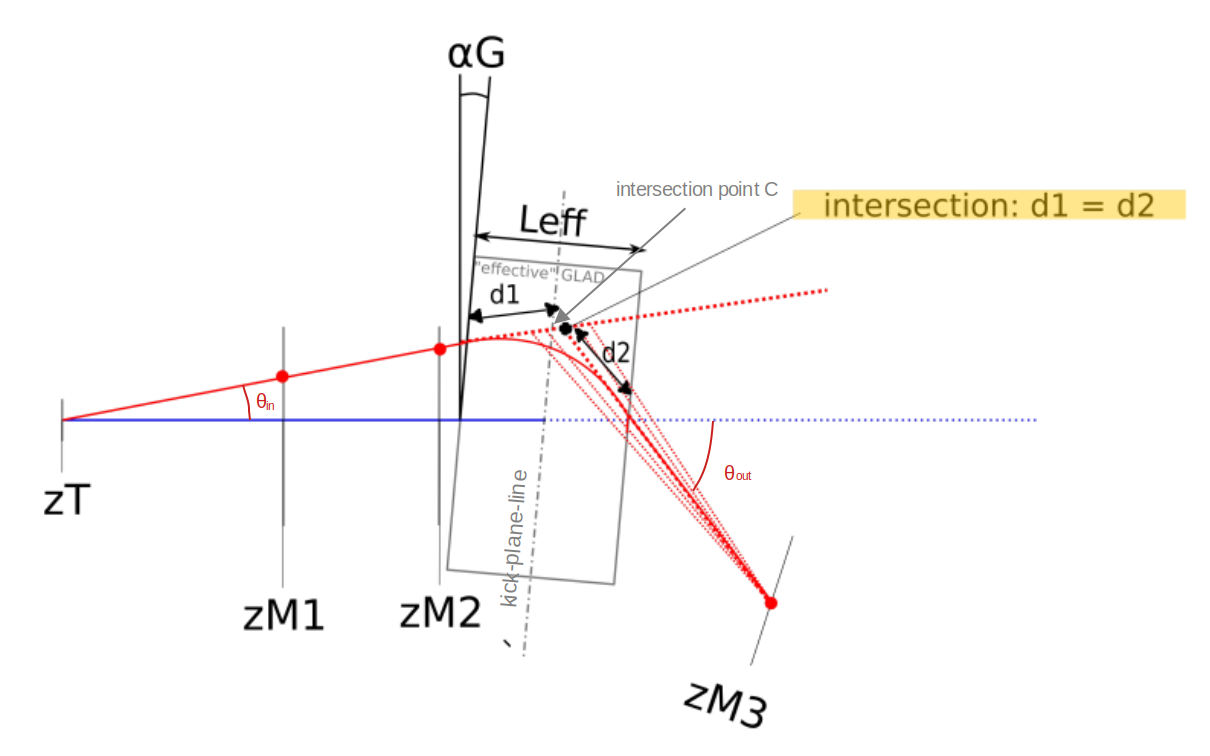
\includegraphics[width=\textwidth]{Figures/kick_point_algorithm.png}
        \caption{First subfigure caption}
        \label{fig:sub1}
    \end{subfigure}
    \hfill % Optional: adds horizontal space between the figures
    % Second subfigure
    \begin{subfigure}[b]{0.45\textwidth}
        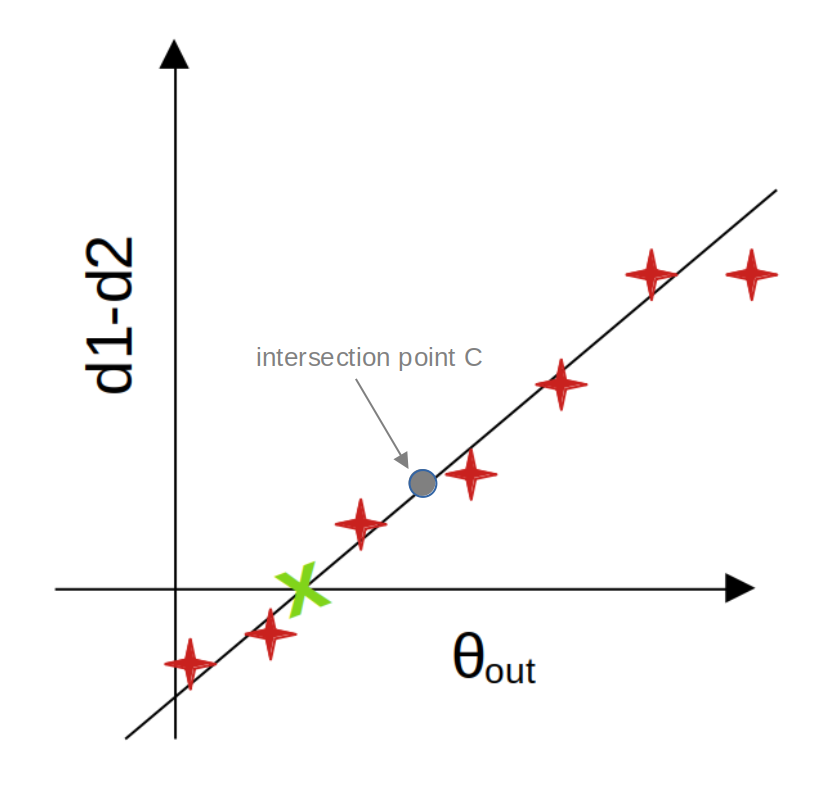
\includegraphics[width=\textwidth]{Figures/intersection_algorithm.png}
        \caption{Second subfigure caption}
        \label{fig:sub2}
    \end{subfigure}

    \caption{Overall figure caption}
    \label{fig:overall}
\end{figure}
\subsection{Event Selection}
no major efforts on th event selection done, look up the code.
\subsection{Fragment Identification}
->order of reconstruction: first fragment, critical! then the two protons

\subsection{QFS-Protons}

\subsection{Reconstruction of excited$ ^{11}$B states}

\subsection{Separation energy, correlation fragment protons, aob..}
